\documentclass[11pt,handout,aspectratio=169]{beamer}


%%%%%%%%% GENERAL PACKAGES
%\usepackage{xcolor}
%\usepackage{pdfpages}
%\usetheme[progressbar=frametitle]{metropolis}
%\setbeamercolor{background canvas}{bg=white}
%\usepackage{appendixnumberbeamer}
%\usepackage{booktabs}
%\usepackage[scale=2]{ccicons}
%\usepackage{pgfplots}
%\usepgfplotslibrary{dateplot}
%\usepackage{xspace}
%\newcommand{\themename}{\textbf{\textsc{metropolis}}\xspace}
%\usepackage[absolute,overlay]{textpos}

%%%%%%%%% COLOR THEME

% Define some colors:
\definecolor{DarkFern}{HTML}{407428}
\definecolor{DarkCharcoal}{HTML}{4D4944}
\definecolor{AlertColor}{RGB}{89,124,158}
\definecolor{HighLight}{RGB}{96,95,134}
\definecolor{Important}{RGB}{234,122,133}
\definecolor{Yellow}{HTML}{00539C}
\colorlet{Fern}{DarkFern!85!white}
\colorlet{Charcoal}{DarkCharcoal!85!white}
\colorlet{LightCharcoal}{Charcoal!50!white}
\colorlet{HighLight2}{AlertColor}
\colorlet{DarkRed}{red!70!black}
\colorlet{DarkBlue}{blue!70!black}
\colorlet{DarkGreen}{green!70!black}
\definecolor{RoyalBlue}{HTML}{00539C}
\definecolor{Peach}{HTML}{EEA47F}
\definecolor{ForestGreen}{HTML}{2C5F2D}
\definecolor{MossGreen}{HTML}{E8FCC9}
% Use the colors:
\setbeamercolor{title}{fg=Fern}
\setbeamercolor{frametitle}{fg=MossGreen,bg=ForestGreen}
\setbeamercolor{normal text}{fg=Charcoal!70!black}
\setbeamercolor{block title}{fg=black,bg=Fern!25!white}
\setbeamercolor{block body}{fg=black,bg=Fern!10!white}
\setbeamercolor{block title alerted}{fg=black,bg=DarkRed!25!white}
\setbeamercolor{block body alerted}{fg=black,bg=DarkRed!10!white}
\setbeamercolor{alerted text}{fg=DarkRed}
\setbeamercolor{itemize item}{fg=Charcoal}



%%%%%%%%% OTHER COMMANDS
\newcommand{\indep}{\perp\!\!\! \perp}
\newcommand{\comment}[1]{}
\newcommand{\bs}{\boldsymbol}
\newcommand{\tr}{\text{trace}}
\newcommand{\sgn}{{\rm sgn}}
\def\T{\top}
%\newcommand{\det}{\text{det}}
\newcommand{\var}{\mathrm{var}}
\newcommand{\cC}{{\cal C}}
\newcommand{\cG}{{\cal G}}
\newcommand{\cV}{{\cal V}}
\newcommand{\cE}{{\cal E}}
\newcommand{\cM}{{\cal M}}
\newcommand{\cP}{{\cal P}}
\newcommand{\cX}{{\cal X}}
\newcommand{\cY}{{\cal Y}}
\newcommand{\X}{\mathbf{X}}
\newcommand{\Y}{\mathbf{Y}}
\newcommand{\x}{\mathbf{x}}
\newcommand{\y}{\mathbf{y}}
\newcommand{\z}{\mathbf{z}}

\newcommand{\argmin}{\operatornamewithlimits{argmin}}
\newcommand{\eps}{\varepsilon}
\newcommand{\<}{\langle}
\renewcommand{\>}{\rangle}


\setbeamertemplate{itemize subitem}{\tiny\raise1.5pt\hbox{\donotcoloroutermaths$\blacktriangleright$}}
\setbeamertemplate{itemize subsubitem}{\tiny\raise1.5pt\hbox{\donotcoloroutermaths$\blacktriangleright$}}
\setbeamertemplate{enumerate item}{\insertenumlabel.}
\setbeamertemplate{enumerate subitem}{\insertenumlabel.\insertsubenumlabel}
\setbeamertemplate{enumerate subsubitem}{\insertenumlabel.\insertsubenumlabel.\insertsubsubenumlabel}
\setbeamertemplate{enumerate mini template}{\insertenumlabel}

\newcommand{\TODO}[1]{{\color{red}{[TODO: #1]}}}


\newcommand{\R}{\mathbb R}
\newcommand{\E}{\mathbb E}
\renewcommand{\P}{\mathbb P}


\DeclareMathOperator*{\cov}{cov}


\newsavebox{\zerobox}
\newenvironment{nospace}
{\par\edef\theprevdepth{\the\prevdepth}\nointerlineskip
  \setbox\zerobox=\vtop to 0pt\bgroup
  \hrule height0pt\kern\dimexpr\baselineskip-\topskip\relax
}
{\par\vss\egroup\ht\zerobox=0pt \wd\zerobox=0pt \dp\zerobox=0pt
  \box\zerobox}

\usepackage{soul}
\makeatletter
\let\HL\hl
\renewcommand\hl{%
  \let\set@color\beamerorig@set@color
  \let\reset@color\beamerorig@reset@color
  \HL}
  \makeatother


\title[STA437-Week1]{STA 437/2005: \\ Methods for Multivariate Data}
\subtitle[]{Weeks 8: Covariance matrix estimation}
\author[Piotr Zwiernik]{Piotr Zwiernik}
\institute[UofT]{University of Toronto}
\date{}


%\usepackage{Sweave}

\begin{document}

\maketitle

\begin{frame}{Covariance matrix estimation}
	We started our discussion of PCA on the population level. 
	\begin{itemize}
		\item maximizing $\bs u^\top \Sigma \bs u$ gives a direction of the highest variance of $X\in \R^m$. \\[5mm]
	\end{itemize}
	
	In practice we have no access to $\Sigma\in \mathbb S^m_+$.\\[5mm]
	
	The main approach is to estimate $\Sigma$ using the sample covariance matrix $S_n$.\\[5mm]
	
	Recall that $S_n$ is almost unbiased.\\[5mm] 
	It can be shown that it is a consistent estimator of $\Sigma$.\\[5mm]
	In other words, if $n$ is ``very large'', $S_n$ should be a good estimator of $\Sigma$.  
\end{frame}

\begin{frame}{High-dimensional problems}
	How large $n$ has to be generally depends on $m$.\\[5mm]
	This is intuitively clear because $\Sigma$ has $\binom{m}{2}=\tfrac{m(m+1)}{2}$ parameters to estimate.\\[5mm]
\alert{Classical asymptotics} lets $n\to \infty$ keeping $m$ fixed. \\[5mm]
\textcolor{blue}{High-dimensional asymptotics} studies estimation when both $m,n\to \infty$.\begin{itemize}
	\item We assume $m/n\to \gamma\in [0,1)$.
\end{itemize}\end{frame}

\begin{frame}{Why does it matter?}
	Suppose that $\Sigma=I_m$. If $S_n$ is close to $\Sigma$ all its eigenvalues should be close to $1$. \\[5mm]
	Consider a simple example: $m=3$, $n=1000$. Sample $S_n$ several times and look at the histogram of eigenvalues. \\
	\begin{minipage}{7cm}
	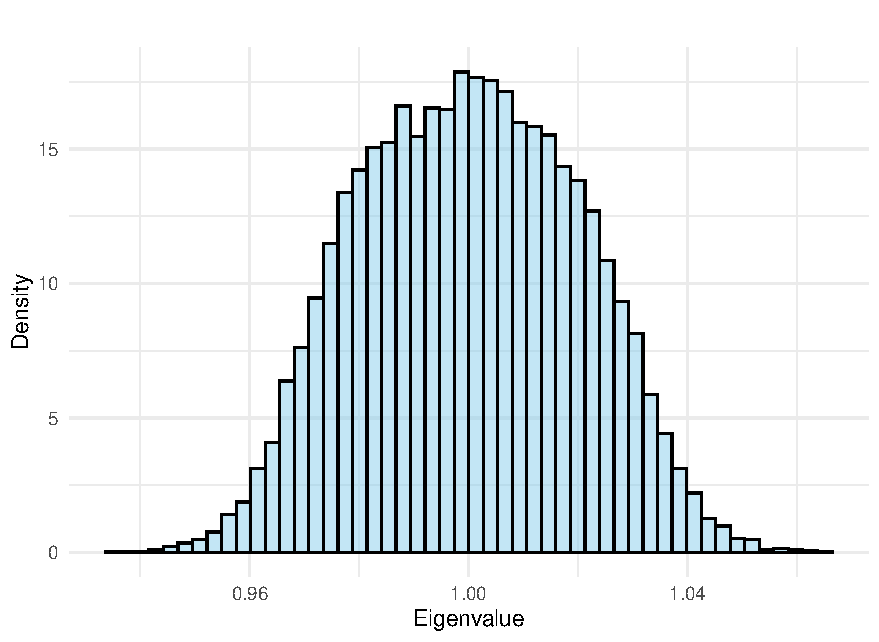
\includegraphics[scale=.45]{pics/HDcov3}		
	\end{minipage}
\begin{minipage}{6.5cm}
	Indeed! A \textbf{sharp} concentration around 1.\\[5mm]
	Arguably, this is a very extreme situation.\\[5mm]
	In typical applications the ration $n/m$ is much smaller. 
\end{minipage}
\end{frame}

\begin{frame}{}
  Consider now the eigenvalue distribution in the same setting but with much higher $m$. \\[5mm]

Take $n=1000$, $m=200$  and $m=500$. 
  \begin{center}
    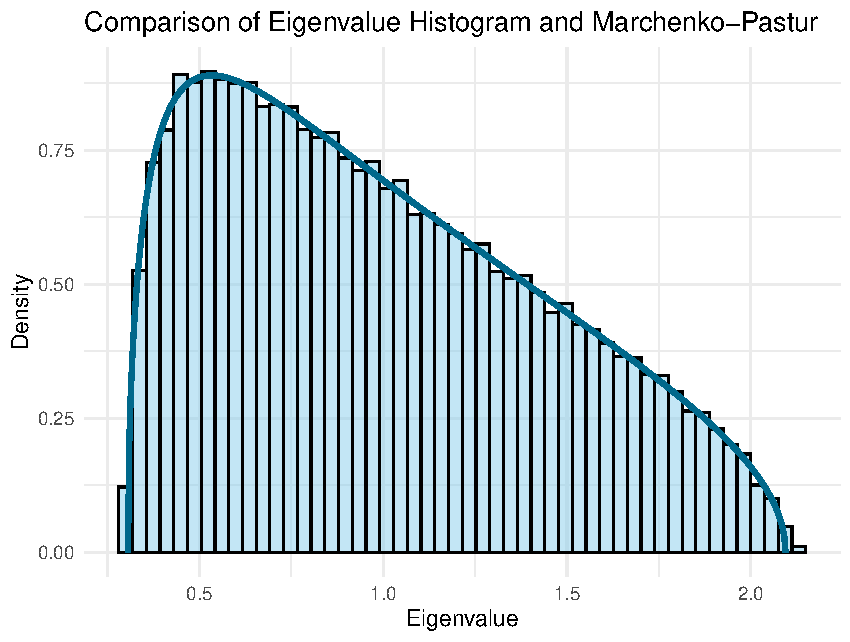
\includegraphics[width=0.45\textwidth]{pics/HDcov1.pdf}
    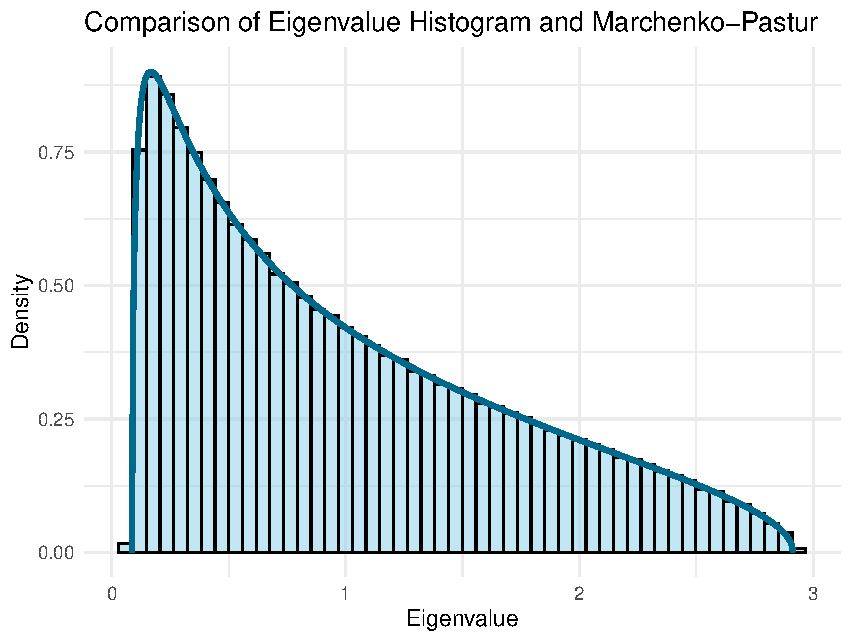
\includegraphics[width=0.45\textwidth]{pics/HDcov2.pdf}
  \end{center}
  The eigenvalues deviate from 1, following the \alert{Marchenko-Pastur law}.
\end{frame}

\begin{frame}{Marchenko-Pastur Law}
Marchenko-Pastur Law gives the limiting distribution of the eigenvalues of $S_n$ ($\Sigma=I_m$) in the limiting case when $m/n \to \gamma$.\\[5mm]

\begin{block}{Marchenko-Pastur Law}
	Let $\lambda_{\min}:=(1-\sqrt{\gamma})^2$, $\lambda_{\max}:=(1+\sqrt{\gamma})^2$. Then MP Law has density
	$$
	f_{\mathrm{MP}}(\lambda) = \frac{1}{2\pi\gamma\lambda}\sqrt{(\lambda_{\max}-\lambda)(\lambda-\lambda_{\min})}\qquad \mbox{for }\lambda\in [\lambda_{\min},\lambda_{\max}].
	$$
\end{block}
\end{frame}

\begin{frame}{Alternative Estimators}
	This example shows that $S_n$ is not a good estimator of $\Sigma$ when $m/n$ is too large.\\[5mm]
	General approach: if there is some additional structure in $\Sigma$, exploit it.
	\begin{itemize}
		\item This stabilizes the estimators.\\[5mm]
	\end{itemize}
	This approach may be problematic if you exploited structure that is not there. \\[5mm]
	We now review some common approaches that work well in a wide-range of scenarios. 
\end{frame}

\begin{frame}{Alternative Estimators Overview}
  \textbf{Linear Shrinkage}: \hl{$\widehat{\Sigma}_{\text{ls}} = (1 - \lambda) S_n + \lambda I_m$} for some $\lambda\in (0,1)$.
  \begin{itemize}
  	\item Reduces variance by shrinking towards $I_m$.\\[5mm]
  \end{itemize}
  
 
  \textbf{Graphical Lasso}: We consider penalized Gaussian log-likelihood. Define
   \[\widehat{K} \;:=\; \arg\min_{K\in \mathbb S^m_+ }\{\textcolor{blue}{\mathrm{tr}(S_nK)-\log\det(K)}+\alert{\lambda\|K\|_1}\},\]
   where $\|K\|_1=\sum_{i\neq j}|K_{ij}|$ ($\ell_1$-penalty). Finally, 
  \hl{$\widehat \Sigma_{\text{glasso}}=\widehat K^{-1}$}.
  \begin{itemize}
  	\item Promotes sparsity in the precision matrix.
  \end{itemize}
\end{frame}

\begin{frame}{Alternative Estimators Continued}
  \textbf{Factor Models}: Suppose $\Sigma$ has the form
  $\Sigma = LL^\top + \Psi$ 
  where $L\in \R^{m\times r}$ for $r<m$ and $\Psi$ is diagonal.
  \begin{itemize}
  	\item We will show how to exploit this in estimation.
  	\item Probabilistic PCA gives one example with $\Psi=\sigma^2 I_m$. \\[5mm]
  \end{itemize}
  
  
  \textbf{Thresholding-Based Methods}: If $\Sigma$ has zeros, it is natural to estimate
  \[\widehat{\Sigma}_{\text{thresh}} = \{(S_n)_{ij} \cdot \mathbb{I}(|(S_n)_{ij}|>\tau)\}_{i,j}.\]
  Sets small covariance entries to zero.
\end{frame}

\begin{frame}{Tyler's Scatter Estimator}
This is a popular estimator in robust statistics. \\[4mm]
If $X\sim E(\bs 0,\Sigma)$ then $Z=\Sigma^{-1/2}X$ is spherical; $Z/\|Z\|$ is uniform on the unit sphere.\\[4mm]
Then $\tfrac1m I_m=\var(Z/\|Z\|)=\E(\tfrac{1}{\|Z\|^2}ZZ^\top)=\E(\tfrac{1}{X^\top \Sigma^{-1}X}\Sigma^{-1/2}XX^\top \Sigma^{-1/2})$.\\[4mm]
Equivalently $\E(\tfrac{1}{X^\top \Sigma^{-1}X}XX^\top)=\tfrac1m \Sigma$. Consider a sample version of this equation:
  \[\sum_{i=1}^n \frac{1}{x^{(i)\top}\Sigma^{-1}x^{(i)}}x^{(i)}x^{(i)\top} = \frac{n}{m}\Sigma.\]
  Under mild conditions, there is a unique solution; computed using fixed-point iterations:
  \[\hat{\Sigma}^{(k+1)} = \frac{m}{n}\sum_{i}\frac{x^{(i)}x^{(i)\top}}{x^{(i)\top}(\hat{\Sigma}^{(k)})^{-1}x^{(i)}}.\]
\end{frame}

\begin{frame}{Summary}
	Estimating the covariance matrix in modern applications raises many challenges. \\[5mm]
	If $\Sigma$ satisfies some structure, we could exploit it to stabilize estimation. \\[5mm]
	We study some structures that can appear in  practice.
	\begin{itemize}
		\item Diagonal plus low rank.
		\item $\Sigma$ or $\Sigma^{-1}$ sparse.\\[5mm]
	\end{itemize}  
	
	This is an active are of research. Links to random matrix theory.
	
\end{frame}

\end{document}

